% Generated from docs/tex/images_benchmark_types/five_examples_metadata.json,
% with additional Type R and Type P defense examples exported from GPT-4o runs.

\subsection*{Conceptual Captions Example}

\begin{figure}[H]
\centering
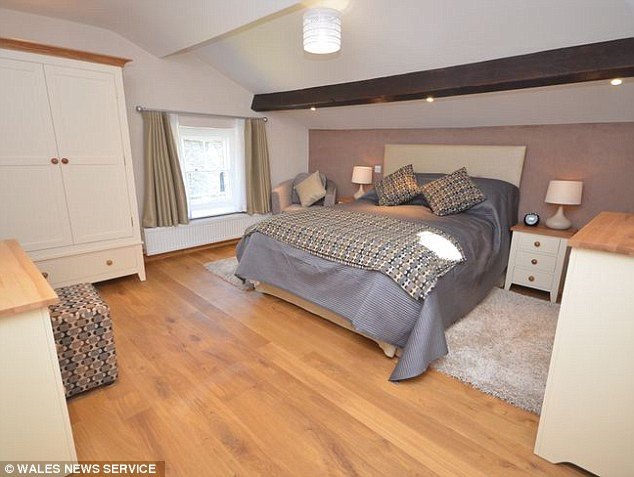
\includegraphics[width=0.70\textwidth]{type_c_conceptual_captions_02.png}
\caption{Conceptual Captions example 2 image sent to the model.}
\end{figure}

\promptbox{\textbf{Prompt for example 2.} Write one concise caption for the image; return only the caption text.}

\resultbox{\textbf{Reference for example 2.} the - bedroom stone cottage can sleep people\\\textbf{GPT-4o response.} Cozy bedroom with wooden flooring and modern decor. (incorrect)\\\textbf{GPT-4o score.} BLEU 0.1604}

\subsection*{FlyingThings3D Example}

\begin{figure}[H]
\centering
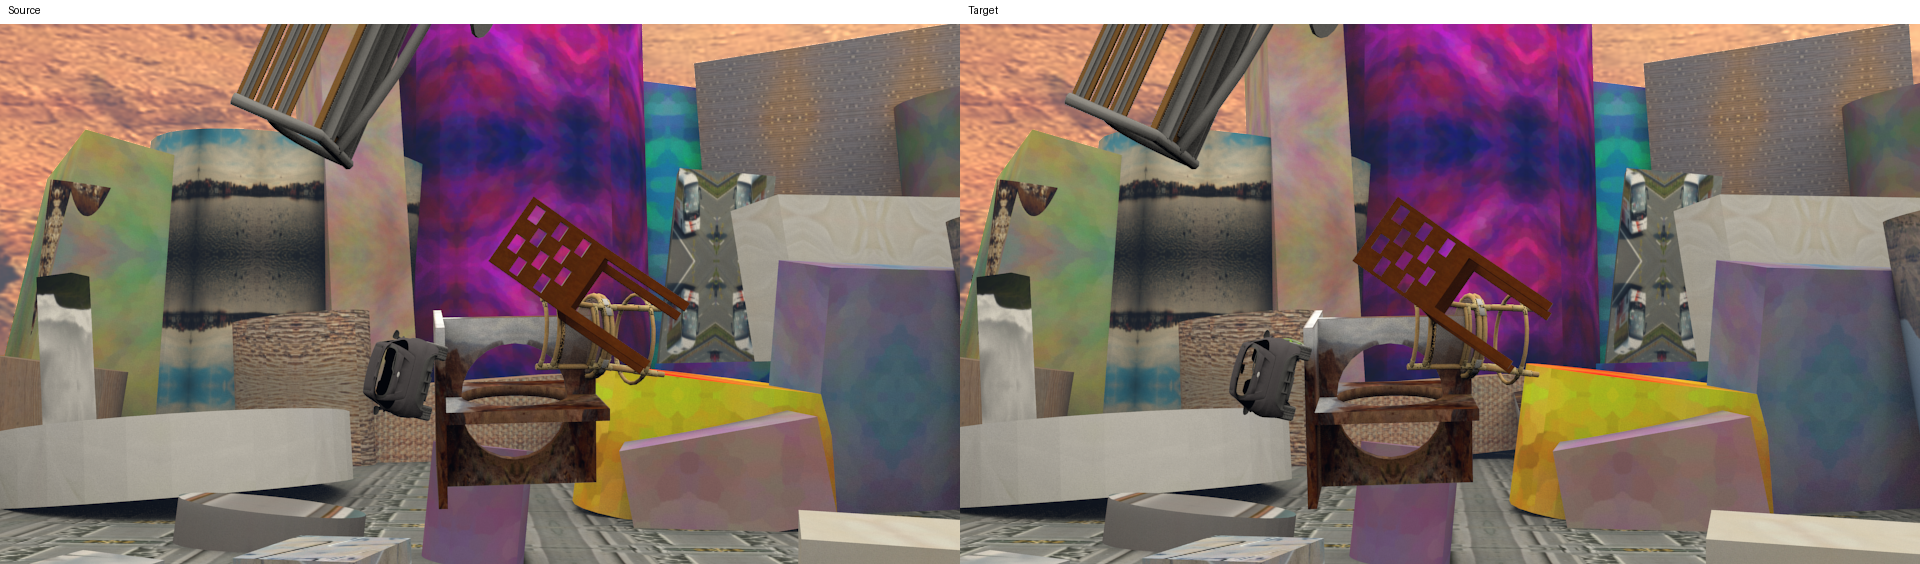
\includegraphics[width=0.70\textwidth]{type_a_flyingthings3d_03.png}
\caption{FlyingThings3D example 3 image sent to the model.}
\end{figure}

\promptbox{\textbf{Prompt for example 3.} Question: What part of the gray car is most visible?\\\textbf{Choices.}\\{} \textbf{A.} the front\\{} \textbf{B. the back}\\{} \textbf{C.} the side\\{} \textbf{D.} the top.}

\resultbox{\textbf{GPT-4o response.} C. the side (incorrect)}

\subsection*{MS COCO Example}

\begin{figure}[H]
\centering
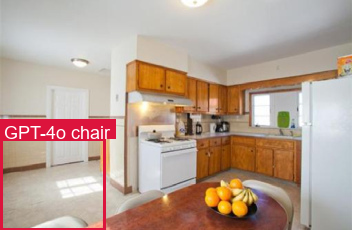
\includegraphics[width=0.70\textwidth]{type_b_mscoco_02_gpt4o_boxes.png}
\caption{MS COCO example 2 image sent to the model with GPT-4o predicted boxes drawn.}
\end{figure}

\promptbox{\textbf{Prompt for example 2.} Target class: chair. Detect every visible instance and return one normalized [x, y, width, height] box per line, or [] if none are visible.}

\resultbox{\textbf{Reference for example 2.} chair\\\textbf{GPT-4o response.} [0.0, 0.6, 0.3, 0.4] (incorrect)\\\textbf{GPT-4o boxes drawn in image.} chair: [0.00, 138.00, 105.60, 230.00]}

\subsection*{HQ-Edit Example}

\begin{figure}[H]
\centering
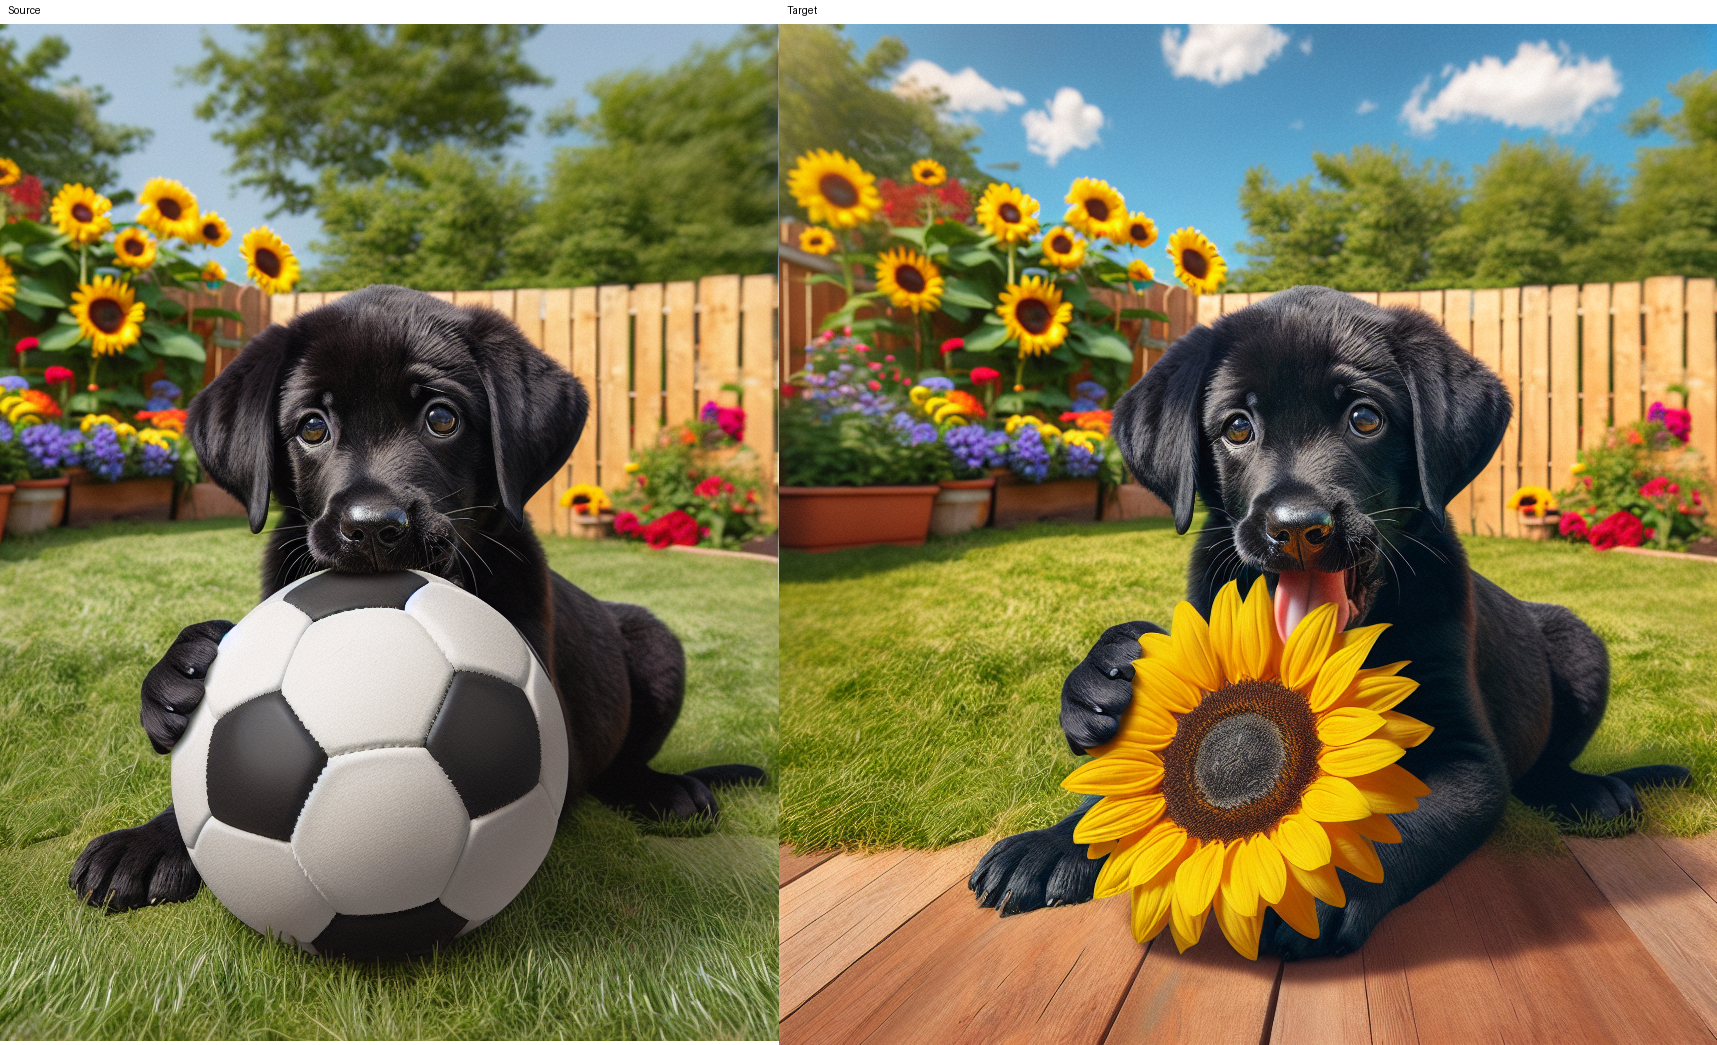
\includegraphics[width=0.70\textwidth]{type_e_hq_edit_05.png}
\caption{HQ-Edit example 5 image sent to the model.}
\end{figure}

\promptbox{\textbf{Prompt for example 5.} Identify which edit instruction produced Image B from Image A.\\\textbf{Choices.}\\{} \textbf{A.} Replace the soccer ball with a miniature sunflower that the puppy is holding in the same manner as the soccer ball.\\{} \textbf{B.} Replace the soccer ball with a miniature sunflower that the kitten is holding in the same manner as the soccer ball.\\{} \textbf{C. Replace the soccer ball with a giant sunflower that the puppy is holding in the same manner as the soccer ball.}\\{} \textbf{D.} Replace the soccer ball with a giant sunflower that the kitten is holding in the same manner as the soccer ball.}

\resultbox{\textbf{GPT-4o response.} C. Replace the soccer ball with a giant sunflower that the puppy is holding in (correct)}

\subsection*{DiffusionDB Example}

\begin{figure}[H]
\centering
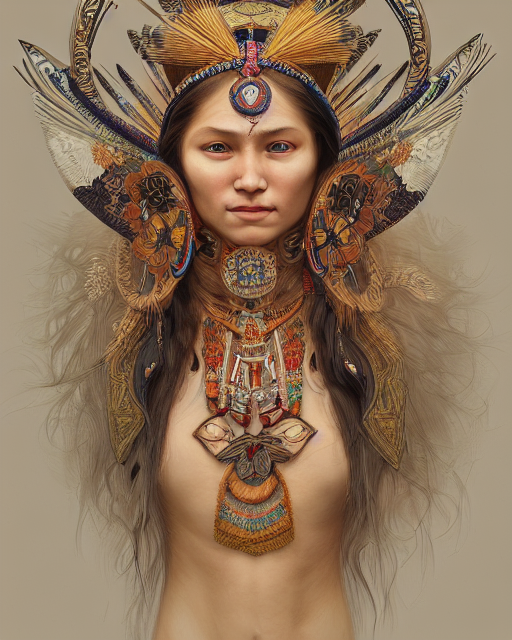
\includegraphics[width=0.70\textwidth]{type_g_diffusiondb_02.png}
\caption{DiffusionDB example 2 image sent to the model.}
\end{figure}

\promptbox{\textbf{Prompt for example 2.} Identify which prompt created the image.\\\textbf{Choices.}\\{} \textbf{A.} a renaissance portrait of dwayne johnson, art in the style of rembrandt!! intricate. ultra detailed, oil on canvas, wet - on - wet technique, pay attention to facial details, highly realistic, cinematic lightning, intricate textures, illusionistic detail,\\{} \textbf{B.} epic 3 d, become legend shiji! gpu mecha controlled by telepathic hackers, made of liquid, bubbles, crystals, and mangroves, houdini sidefx, perfect render, artstation trending, by jeremy mann, tsutomi nihei and ilya kuvshinov\\{} \textbf{C.} an airbrush painting of cyber war machine scene in area 5 1 by destiny womack, gregoire boonzaier, harrison fisher, richard dadd\\{} \textbf{D. portrait of a dancing eagle woman, beautiful blonde haired lakota sioux goddess, intricate, highly detailed art by james jean, ray tracing, digital painting, artstation, concept art, smooth, sharp focus, illustration, artgerm and greg rutkowski and alphonse mucha, vladimir kush, giger, 8 k.}}

\resultbox{\textbf{GPT-4o response.} D (correct)}

\subsection*{ImageNet Example}

\begin{figure}[H]
\centering
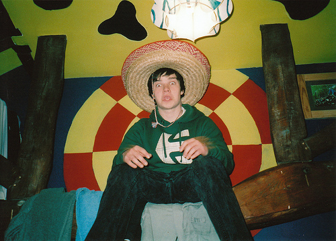
\includegraphics[width=0.70\textwidth]{type_l_imagenet1k_01.png}
\caption{ImageNet example 1 image sent to the model.}
\end{figure}

\promptbox{\textbf{Prompt for example 1.} Return exactly one label from the complete ImageNet-1K label list.}

\resultbox{\textbf{Reference for example 1.} sombrero\\\textbf{GPT-4o response.} sombrero (correct)}

\subsection*{TAD66K Rating Example}

\begin{figure}[H]
\centering
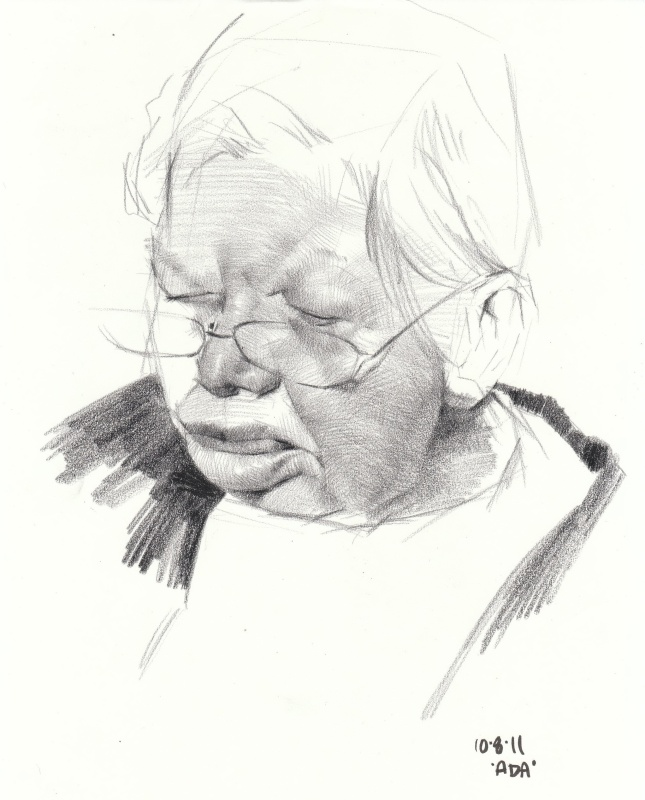
\includegraphics[width=0.70\textwidth]{type_r_tad66k_06.png}
\caption{TAD66K rating example 6 image sent to the model.}
\end{figure}

\promptbox{\textbf{Prompt for example 6.} Rate the overall aesthetic quality of this image from 1 to 10, where 1 is very poor and 10 is exceptional. Return exactly one integer from 1 to 10.}

\resultbox{\textbf{Reference for example 6.} 7\\\textbf{GPT-4o response.} 7 (correct)\\\textbf{GPT-4o absolute error.} 0}

\subsection*{Pick-a-Pic Preference Example}

\begin{figure}[H]
\centering
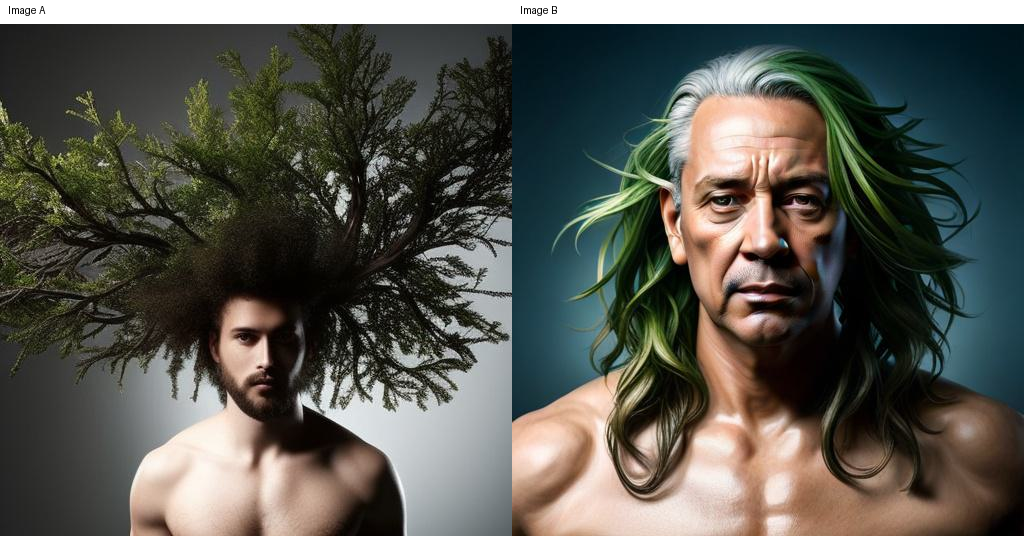
\includegraphics[width=0.70\textwidth]{type_p_pick_a_pic_04.png}
\caption{Pick-a-Pic preference example 4 image pair sent to the model.}
\end{figure}

\promptbox{\textbf{Prompt for example 4.} Which image is more aesthetically pleasing overall?\\\textbf{Choices.}\\{} \textbf{A.} Image A\\{} \textbf{B.} Image B\\{} Return only A or B.}

\resultbox{\textbf{Reference for example 4.} Image A\\\textbf{GPT-4o response.} A (correct)}
